% Clean hierarchical redraw of plots/mismatch/2_1/geneTree_2_1.gml
% This is the ORIGINAL gene tree, before generateHybridNetwork() subdivided
% edges (553360->12) and (550480->14) and inserted the hybridization edge
% -- compare against hybrid_network_2_1_clean.tex.
% Compile with: pdflatex geneTree_2_1_clean.tex
\documentclass{article}
\usepackage[margin=1cm]{geometry}
\usepackage{tikz}
\usetikzlibrary{arrows.meta}

% matplotlib tab:blue / tab:orange, matching the gene_color values in the GML
\definecolor{tabblue}{rgb}{0.12156863,0.46666667,0.70588235}
\definecolor{taborange}{rgb}{1.0,0.49803922,0.05490196}

\begin{document}
\thispagestyle{empty}
\begin{center}
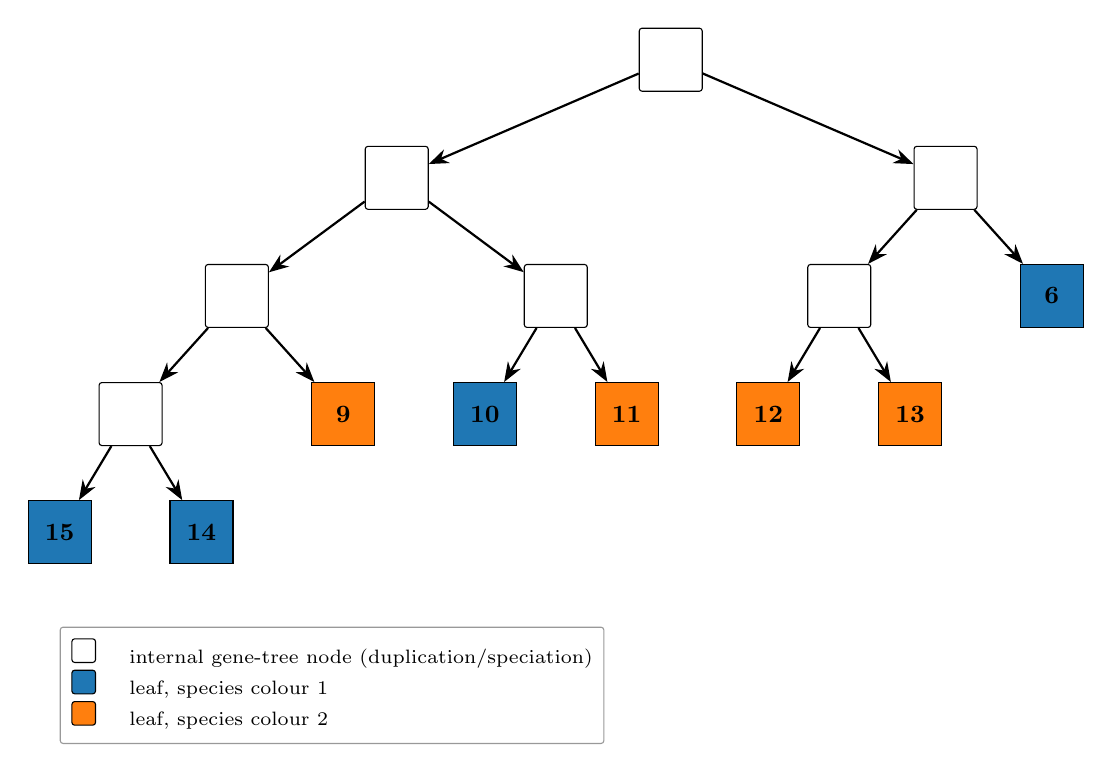
\begin{tikzpicture}[
  >={Stealth[length=2.5mm]},
  every node/.style={font=\small\bfseries},
  internal/.style={rectangle, fill=white, text=black, minimum size=8mm, draw=black, rounded corners=1pt},
  leafblue/.style={rectangle, fill=tabblue, text=black, minimum size=8mm, draw=black},
  leaforange/.style={rectangle, fill=taborange, text=black, minimum size=8mm, draw=black},
  treeedge/.style={->, thick},
]

% ---- depth 0: root ----
\node[internal] (v1) at (7.76, 0)    {};

% ---- depth 1 ----
\node[internal] (v2) at (4.28, -1.5) {};
\node[internal] (v3) at (11.25, -1.5){};

% ---- depth 2 ----
\node[internal]   (v4) at (2.25, -3) {};
\node[internal]   (v5) at (6.3, -3)  {};
\node[internal]   (v6) at (9.9, -3)  {};
\node[leafblue]   (l6) at (12.6, -3) {6};

% ---- depth 3 ----
\node[internal]   (v7)  at (0.9, -4.5) {};
\node[leaforange] (l9)  at (3.6, -4.5) {9};
\node[leafblue]   (l10) at (5.4, -4.5) {10};
\node[leaforange] (l11) at (7.2, -4.5) {11};
\node[leaforange] (l12) at (9.0, -4.5) {12};
\node[leaforange] (l13) at (10.8, -4.5){13};

% ---- depth 4 ----
\node[leafblue]   (l15) at (0.0, -6) {15};
\node[leafblue]   (l14) at (1.8, -6) {14};

% ---- edges (exactly as in geneTree_2_1.gml) ----
\draw[treeedge] (v1) -- (v2);
\draw[treeedge] (v1) -- (v3);
\draw[treeedge] (v2) -- (v4);
\draw[treeedge] (v2) -- (v5);
\draw[treeedge] (v3) -- (v6);
\draw[treeedge] (v3) -- (l6);
\draw[treeedge] (v4) -- (v7);
\draw[treeedge] (v4) -- (l9);
\draw[treeedge] (v5) -- (l10);
\draw[treeedge] (v5) -- (l11);
\draw[treeedge] (v6) -- (l12);
\draw[treeedge] (v6) -- (l13);
\draw[treeedge] (v7) -- (l15);
\draw[treeedge] (v7) -- (l14);

% ---- legend ----
\node[anchor=north west, font=\scriptsize, align=left, draw=black!40, fill=white, inner sep=4pt, rounded corners=1pt]
  at (0.0, -7.2) {%
  \begin{tabular}{@{}ll@{}}
    \tikz\node[internal, minimum size=3mm]{}; & internal gene-tree node (duplication/speciation) \\
    \tikz\node[leafblue, minimum size=3mm]{};   & leaf, species colour 1 \\
    \tikz\node[leaforange, minimum size=3mm]{}; & leaf, species colour 2 \\
  \end{tabular}%
};

\end{tikzpicture}
\end{center}
\end{document}
